\documentclass[8pt,aspectratio=169]{beamer}
\usetheme{Madrid}
\usecolortheme{seahorse}
\setbeamertemplate{navigation symbols}{}

\usepackage{graphicx}
\usepackage{booktabs}
\usepackage{adjustbox}
\usepackage{multicol}
\usepackage{amsmath}
\usepackage{amssymb}
\usepackage{algorithm2e}
\usepackage{tcolorbox}
\usepackage{listings}
\usepackage{tikz}
\usetikzlibrary{shapes.geometric, arrows, positioning}

% Code formatting
\lstset{
    language=Python,
    basicstyle=\ttfamily\tiny,
    keywordstyle=\color{blue},
    stringstyle=\color{red},
    commentstyle=\color{green!50!black},
    breaklines=true,
    frame=single,
    numbers=left,
    numberstyle=\tiny\color{gray}
}

% Custom commands
\newcommand{\given}{\mid}
\newcommand{\prob}[1]{P(#1)}
\newcommand{\highlight}[1]{\textcolor{blue}{\textbf{#1}}}

\title{Generating Shakespeare Sonnets with N-Gram Language Models}
\subtitle{Natural Language Processing - Week 1 Extension}
\author{BSc Computer Science}
\date{2025}

\begin{document}

\frame{\titlepage}

% Outline
\begin{frame}{Session Outline}
\begin{columns}[T]
\column{0.45\textwidth}
\textbf{Theory (25 min)}
\begin{itemize}
    \item Shakespeare's sonnets: Structure \& style
    \item N-gram models for poetry
    \item Special challenges in poetry generation
    \item Evaluation metrics for generated text
\end{itemize}

\column{0.45\textwidth}
\textbf{Practice (25 min)}
\begin{itemize}
    \item Text preprocessing for sonnets
    \item Building n-gram models
    \item Generation techniques
    \item Hands-on: Generate your own sonnets
\end{itemize}
\end{columns}

\vspace{0.5em}
\begin{tcolorbox}[colback=blue!5!white,colframe=blue!75!black]
\textbf{Learning Goals:} Apply n-gram models to creative text generation, understand domain-specific challenges
\end{tcolorbox}
\end{frame}

% Part 1: Shakespeare Background
\begin{frame}{Shakespeare's Sonnets: Literary Context}
\begin{columns}[T]
\column{0.5\textwidth}
\textbf{Historical Background}
\begin{itemize}
    \item 154 sonnets published in 1609
    \item Written over ~20 year period
    \item Themes: love, beauty, mortality, time
    \item Revolutionary use of English
\end{itemize}

\vspace{0.5em}
\textbf{Why Study with NLP?}
\begin{itemize}
    \item Rich, structured language patterns
    \item Fixed poetic form (constraints)
    \item Historical importance
    \item Challenging generation task
\end{itemize}

\column{0.45\textwidth}
\begin{tcolorbox}[colback=green!5!white,colframe=green!75!black,title=Sonnet 18]
\tiny
Shall I compare thee to a summer's day?\\
Thou art more lovely and more temperate:\\
Rough winds do shake the darling buds of May,\\
And summer's lease hath all too short a date:\\
Sometime too hot the eye of heaven shines,\\
And often is his gold complexion dimm'd;\\
And every fair from fair sometime declines,\\
By chance, or nature's changing course untrimm'd;\\
But thy eternal summer shall not fade\\
Nor lose possession of that fair thou owest;\\
Nor shall Death brag thou wander'st in his shade,\\
When in eternal lines to time thou growest:\\
So long as men can breathe, or eyes can see,\\
So long lives this, and this gives life to thee.
\end{tcolorbox}
\end{columns}
\end{frame}

% Sonnet Structure
\begin{frame}{Sonnet Structure: The Shakespearean Form}
\begin{columns}[T]
\column{0.55\textwidth}
\textbf{Formal Requirements}
\begin{enumerate}
    \item \textbf{14 lines} exactly
    \item \textbf{Iambic pentameter}: 10 syllables per line
    \begin{itemize}
        \item Pattern: da-DUM da-DUM da-DUM da-DUM da-DUM
        \item Example: ``Shall I / com-PARE / thee TO / a SUM / mer's DAY?''
    \end{itemize}
    \item \textbf{Rhyme scheme}: ABAB CDCD EFEF GG
    \item \textbf{Volta}: Thematic turn at line 9
    \item \textbf{Couplet}: Final two lines summarize/resolve
\end{enumerate}

\column{0.4\textwidth}
\begin{tcolorbox}[colback=yellow!5!white,colframe=yellow!75!black,title=Structure Visualization]
\centering
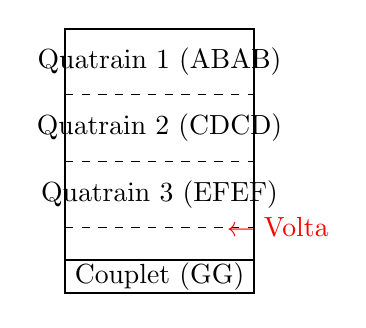
\begin{tikzpicture}[scale=0.6]
\draw[thick] (0,0) rectangle (4,5.6);
\draw[dashed] (0,4.2) -- (4,4.2);
\draw[dashed] (0,2.8) -- (4,2.8);
\draw[dashed] (0,1.4) -- (4,1.4);
\draw[thick] (0,0.7) -- (4,0.7);
\node at (2,4.9) {Quatrain 1 (ABAB)};
\node at (2,3.5) {Quatrain 2 (CDCD)};
\node at (2,2.1) {Quatrain 3 (EFEF)};
\node at (2,0.35) {Couplet (GG)};
\node[red] at (4.5,1.4) {$\leftarrow$ Volta};
\end{tikzpicture}
\end{tcolorbox}

\vspace{0.3em}
\textbf{Computational Challenges:}
\begin{itemize}
    \item Maintaining meter while being coherent
    \item Enforcing rhyme without repetition
    \item Balancing structure with creativity
\end{itemize}
\end{columns}
\end{frame}

% Language Characteristics
\begin{frame}{Shakespearean Language Characteristics}
\begin{columns}[T]
\column{0.48\textwidth}
\textbf{Vocabulary Features}
\begin{itemize}
    \item \textbf{Archaic forms}: thee, thou, thy, thine, hath, doth
    \item \textbf{Contractions}: o'er, e'er, 'tis, ne'er
    \item \textbf{Inversions}: ``Rough winds do shake'' vs ``Rough winds shake''
    \item \textbf{Rich vocabulary}: ~31,000 unique words in complete works
\end{itemize}

\vspace{0.3em}
\textbf{Statistical Properties}
\begin{itemize}
    \item Average sentence length: 12-15 words
    \item Vocabulary richness: Type-Token Ratio $\approx$ 0.45
    \item Most frequent words: thou, thy, thee, love, time
\end{itemize}

\column{0.48\textwidth}
\begin{tcolorbox}[colback=orange!5!white,colframe=orange!75!black,title=Word Frequency Analysis]
\centering
\includegraphics[width=\textwidth]{figures/shakespeare_word_freq.pdf}
\end{tcolorbox}

\textbf{Implications for N-grams:}
\begin{itemize}
    \item Need larger context (3-grams or higher)
    \item Special handling of archaic forms
    \item Preserve poetic inversions
\end{itemize}
\end{columns}
\end{frame}

% N-gram Models for Poetry
\begin{frame}{N-Gram Models for Poetry Generation}
\begin{columns}[T]
\column{0.55\textwidth}
\textbf{Why N-grams Work for Poetry}
\begin{itemize}
    \item Capture local word dependencies
    \item Learn stylistic patterns
    \item Preserve author's ``voice''
    \item Computationally simple
\end{itemize}

\vspace{0.3em}
\textbf{Model Selection}
\begin{tabular}{lll}
\toprule
Model & Pros & Cons \\
\midrule
Unigram & Fast & No context \\
Bigram & Some context & Limited memory \\
Trigram & Good balance & Sparse data \\
4-gram+ & Rich context & Very sparse \\
\bottomrule
\end{tabular}

\vspace{0.3em}
\textbf{Poetry-Specific Modifications}
\begin{itemize}
    \item Line-aware generation
    \item Rhyme dictionary integration
    \item Syllable counting
    \item Meter checking
\end{itemize}

\column{0.4\textwidth}
\begin{tcolorbox}[colback=blue!5!white,colframe=blue!75!black,title=Generation Pipeline]
\centering
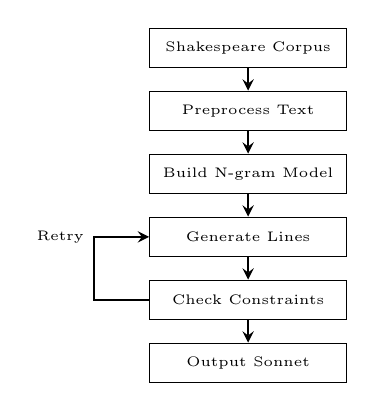
\begin{tikzpicture}[scale=0.7, node distance=0.8cm]
\tikzstyle{box} = [rectangle, draw, minimum width=2.5cm, minimum height=0.5cm, text centered, font=\tiny]
\tikzstyle{arrow} = [thick,->,>=stealth]

\node[box] (corpus) {Shakespeare Corpus};
\node[box, below of=corpus] (preprocess) {Preprocess Text};
\node[box, below of=preprocess] (ngram) {Build N-gram Model};
\node[box, below of=ngram] (generate) {Generate Lines};
\node[box, below of=generate] (check) {Check Constraints};
\node[box, below of=check] (output) {Output Sonnet};

\draw[arrow] (corpus) -- (preprocess);
\draw[arrow] (preprocess) -- (ngram);
\draw[arrow] (ngram) -- (generate);
\draw[arrow] (generate) -- (check);
\draw[arrow] (check) -- (output);
\draw[arrow] (check.west) -- ++(-1,0) |- (generate.west) node[midway,left,font=\tiny] {Retry};
\end{tikzpicture}
\end{tcolorbox}
\end{columns}
\end{frame}

% Text Preprocessing
\begin{frame}[fragile]{Text Preprocessing for Sonnets}
\begin{columns}[T]
\column{0.52\textwidth}
\textbf{Preprocessing Pipeline}
\begin{lstlisting}[language=Python]
def preprocess_sonnet(text):
    # 1. Basic cleaning
    text = text.lower()
    text = re.sub(r'[^\w\s\']', '', text)
    
    # 2. Handle contractions
    contractions = {
        "o'er": "over",
        "'tis": "it is",
        "ne'er": "never"
    }
    for old, new in contractions.items():
        text = text.replace(old, new)
    
    # 3. Tokenization
    tokens = text.split()
    
    # 4. Add line markers
    lines = text.split('\n')
    processed = []
    for line in lines:
        tokens = ['<START>'] + line.split() + ['<END>']
        processed.extend(tokens)
    
    return processed
\end{lstlisting}

\column{0.43\textwidth}
\textbf{Special Considerations}
\begin{itemize}
    \item \textbf{Preserve line structure}: Add START/END tokens
    \item \textbf{Handle punctuation}: Keep apostrophes, remove others
    \item \textbf{Case sensitivity}: Lowercase for matching
    \item \textbf{Archaic forms}: Standardize or preserve?
\end{itemize}

\vspace{0.3em}
\begin{tcolorbox}[colback=red!5!white,colframe=red!75!black,title=Common Issues]
\small
\begin{itemize}
    \item \textbf{Over-preprocessing}: Losing poetic structure
    \item \textbf{Under-preprocessing}: Too many unique tokens
    \item \textbf{Balance}: Preserve style while ensuring generation quality
\end{itemize}
\end{tcolorbox}
\end{columns}
\end{frame}

% Building the N-gram Model
\begin{frame}[fragile]{Building the N-gram Model}
\begin{columns}[T]
\column{0.55\textwidth}
\textbf{Implementation}
\begin{lstlisting}[language=Python]
from collections import defaultdict, Counter

def build_ngram_model(tokens, n=3):
    model = defaultdict(Counter)
    
    # Create n-grams
    for i in range(len(tokens) - n):
        context = tuple(tokens[i:i+n-1])
        next_word = tokens[i+n-1]
        model[context][next_word] += 1
    
    # Convert to probabilities
    for context in model:
        total = sum(model[context].values())
        for word in model[context]:
            model[context][word] /= total
    
    return model

# Example usage
tokens = preprocess_sonnets(shakespeare_text)
bigram_model = build_ngram_model(tokens, n=2)
trigram_model = build_ngram_model(tokens, n=3)
\end{lstlisting}

\column{0.4\textwidth}
\textbf{Model Statistics}
\begin{itemize}
    \item \textbf{Corpus size}: 154 sonnets
    \item \textbf{Total tokens}: ~17,000
    \item \textbf{Unique tokens}: ~3,000
    \item \textbf{Unique bigrams}: ~8,000
    \item \textbf{Unique trigrams}: ~12,000
\end{itemize}

\vspace{0.3em}
\begin{tcolorbox}[colback=green!5!white,colframe=green!75!black,title=Smoothing Techniques]
\small
For unseen n-grams:
\begin{itemize}
    \item \textbf{Add-one}: Add 1 to all counts
    \item \textbf{Good-Turing}: Redistribute probability mass
    \item \textbf{Backoff}: Fall back to (n-1)-gram
\end{itemize}
\end{tcolorbox}
\end{columns}
\end{frame}

% Generation Techniques
\begin{frame}[fragile]{Generation Techniques}
\begin{columns}[T]
\column{0.58\textwidth}
\textbf{Basic Generation}
\begin{lstlisting}[language=Python]
def generate_line(model, n=3, max_words=10):
    # Select good starting context
    starters = [ctx for ctx in model.keys()
                if ctx[0] in ['when', 'shall', 'thy']]
    
    context = random.choice(starters)
    line = list(context)
    
    for _ in range(max_words - n + 1):
        if context not in model:
            break
        
        # Weighted random selection
        next_words = model[context]
        words = list(next_words.keys())
        probs = list(next_words.values())
        
        next_word = np.random.choice(words, p=probs)
        line.append(next_word)
        
        # Update context
        context = tuple(line[-(n-1):])
        
        if next_word == '<END>':
            break
    
    return ' '.join(line)
\end{lstlisting}

\column{0.38\textwidth}
\textbf{Advanced Techniques}

\begin{itemize}
    \item \textbf{Temperature sampling}:
    \begin{itemize}
        \item Adjust randomness
        \item $P'(w) = \frac{P(w)^{1/T}}{\sum P(w_i)^{1/T}}$
    \end{itemize}
    \item \textbf{Beam search}:
    \begin{itemize}
        \item Keep top-k candidates
        \item Select best complete line
    \end{itemize}
    \item \textbf{Constrained generation}:
    \begin{itemize}
        \item Force rhyme words
        \item Count syllables
        \item Check meter
    \end{itemize}
\end{itemize}

\vspace{0.3em}
\begin{tcolorbox}[colback=yellow!5!white,colframe=yellow!75!black]
\small
\textbf{Tip}: Start with simple generation, then add constraints gradually
\end{tcolorbox}
\end{columns}
\end{frame}

% Handling Rhyme
\begin{frame}[fragile]{Implementing Rhyme Constraints}
\begin{columns}[T]
\column{0.55\textwidth}
\textbf{Rhyme Detection}
\begin{lstlisting}[language=Python]
def get_rhyme_sound(word):
    """Extract rhyme sound (simplified)"""
    # Real implementation would use CMU Pronouncing Dict
    endings = {
        'ay': ['day', 'may', 'say', 'way'],
        'ight': ['night', 'light', 'sight', 'might'],
        'ove': ['love', 'dove', 'above'],
        'ime': ['time', 'rhyme', 'chime']
    }
    
    for sound, words in endings.items():
        if word in words:
            return sound
    return None

def generate_rhyming_line(model, rhyme_with):
    """Generate line that rhymes with given word"""
    rhyme_sound = get_rhyme_sound(rhyme_with)
    candidates = []
    
    for _ in range(100):  # Try multiple times
        line = generate_line(model)
        last_word = line.split()[-1]
        if get_rhyme_sound(last_word) == rhyme_sound:
            candidates.append(line)
    
    return random.choice(candidates) if candidates else None
\end{lstlisting}

\column{0.4\textwidth}
\textbf{ABAB CDCD EFEF GG Pattern}

\begin{tcolorbox}[colback=blue!5!white,colframe=blue!75!black]
\small
\begin{enumerate}
    \item Generate line 1 freely (A)
    \item Generate line 2 freely (B)
    \item Generate line 3 rhyming with 1 (A)
    \item Generate line 4 rhyming with 2 (B)
    \item Repeat for next quatrains
    \item Final couplet: two rhyming lines
\end{enumerate}
\end{tcolorbox}

\vspace{0.3em}
\textbf{Challenges}
\begin{itemize}
    \item Limited rhyming vocabulary
    \item Maintaining coherence
    \item Avoiding forced rhymes
    \item Balancing rhyme with meaning
\end{itemize}
\end{columns}
\end{frame}

% Evaluation Metrics
\begin{frame}{Evaluating Generated Sonnets}
\begin{columns}[T]
\column{0.5\textwidth}
\textbf{Quantitative Metrics}
\begin{itemize}
    \item \textbf{Perplexity}: How well model predicts next word
    $$PPL = 2^{-\frac{1}{N}\sum_{i=1}^{N} \log_2 P(w_i|context)}$$
    \item \textbf{BLEU Score}: Compare with real sonnets
    \item \textbf{Rhyme accuracy}: \% correct rhymes
    \item \textbf{Meter compliance}: \% correct rhythm
    \item \textbf{Vocabulary diversity}: Type-Token Ratio
\end{itemize}

\vspace{0.3em}
\textbf{Qualitative Assessment}
\begin{itemize}
    \item Coherence and meaning
    \item Poetic quality
    \item Style consistency
    \item Creativity/originality
\end{itemize}

\column{0.45\textwidth}
\begin{tcolorbox}[colback=green!5!white,colframe=green!75!black,title=Evaluation Results]
\centering
\includegraphics[width=\textwidth]{figures/sonnet_evaluation.pdf}
\end{tcolorbox}

\begin{tcolorbox}[colback=yellow!5!white,colframe=yellow!75!black]
\small
\textbf{Human Evaluation}: Best judge of poetic quality
\begin{itemize}
    \item Turing test: Can readers distinguish from real?
    \item Preference ranking
    \item Specific feedback on issues
\end{itemize}
\end{tcolorbox}
\end{columns}
\end{frame}

% Common Problems and Solutions
\begin{frame}{Common Problems and Solutions}
\begin{columns}[T]
\column{0.48\textwidth}
\textbf{Problem 1: Repetitive Output}
\begin{itemize}
    \item \textbf{Symptom}: Same phrases repeatedly
    \item \textbf{Cause}: High-probability sequences dominate
    \item \textbf{Solutions}:
    \begin{itemize}
        \item Temperature sampling
        \item Penalty for recently used words
        \item Diverse starting contexts
    \end{itemize}
\end{itemize}

\vspace{0.3em}
\textbf{Problem 2: Incoherent Lines}
\begin{itemize}
    \item \textbf{Symptom}: Grammatically wrong or nonsensical
    \item \textbf{Cause}: Limited context in bigrams
    \item \textbf{Solutions}:
    \begin{itemize}
        \item Use trigrams or higher
        \item Add syntax checking
        \item Post-process filtering
    \end{itemize}
\end{itemize}

\column{0.48\textwidth}
\textbf{Problem 3: Poor Rhyming}
\begin{itemize}
    \item \textbf{Symptom}: Forced or missing rhymes
    \item \textbf{Cause}: Limited rhyming vocabulary
    \item \textbf{Solutions}:
    \begin{itemize}
        \item Pre-compute rhyme sets
        \item Generate multiple candidates
        \item Relax exact rhyme requirement
    \end{itemize}
\end{itemize}

\vspace{0.3em}
\textbf{Problem 4: Wrong Meter}
\begin{itemize}
    \item \textbf{Symptom}: Lines too long/short
    \item \textbf{Cause}: No syllable counting
    \item \textbf{Solutions}:
    \begin{itemize}
        \item Add syllable dictionary
        \item Generate with constraints
        \item Post-generation filtering
    \end{itemize}
\end{itemize}
\end{columns}

\vspace{0.3em}
\begin{tcolorbox}[colback=red!5!white,colframe=red!75!black]
\textbf{Key Insight}: Balance between structure and creativity - too many constraints kill creativity, too few produce nonsense
\end{tcolorbox}
\end{frame}

% Visualization and Analysis
\begin{frame}{Visualizing Model Behavior}
\begin{columns}[T]
\column{0.48\textwidth}
\centering
\includegraphics[width=\textwidth]{figures/ngram_distribution.pdf}

\vspace{0.3em}
\includegraphics[width=\textwidth]{figures/generation_probability.pdf}

\column{0.48\textwidth}
\centering
\includegraphics[width=\textwidth]{figures/vocabulary_coverage.pdf}

\vspace{0.3em}
\textbf{Key Observations}
\begin{itemize}
    \item Power law distribution of n-grams
    \item Most contexts have few continuations
    \item 20\% of vocabulary covers 80\% of usage
    \item Trigrams capture more style than bigrams
\end{itemize}
\end{columns}
\end{frame}

% Practical Exercise
\begin{frame}[fragile]{Hands-On Exercise: Generate Your First Sonnet}
\begin{columns}[T]
\column{0.55\textwidth}
\textbf{Step-by-Step Implementation}
\begin{lstlisting}[language=Python]
# 1. Load and preprocess sonnets
sonnets = load_shakespeare_sonnets()
tokens = preprocess_sonnets(sonnets)

# 2. Build models
bigram = build_ngram_model(tokens, n=2)
trigram = build_ngram_model(tokens, n=3)

# 3. Generate a quatrain
def generate_quatrain(model):
    lines = []
    # Generate ABAB pattern
    lines.append(generate_line(model))  # A
    lines.append(generate_line(model))  # B
    lines.append(generate_rhyming_line(model, 
                 get_last_word(lines[0])))  # A
    lines.append(generate_rhyming_line(model,
                 get_last_word(lines[1])))  # B
    return lines

# 4. Complete sonnet
quatrain1 = generate_quatrain(trigram)
quatrain2 = generate_quatrain(trigram)
quatrain3 = generate_quatrain(trigram)
couplet = generate_couplet(trigram)

sonnet = quatrain1 + quatrain2 + quatrain3 + couplet
\end{lstlisting}

\column{0.4\textwidth}
\textbf{Try These Experiments}
\begin{enumerate}
    \item \textbf{Compare n-gram orders}: 
    \begin{itemize}
        \item Generate with bigram vs trigram
        \item Which sounds more Shakespearean?
    \end{itemize}
    \item \textbf{Temperature variation}:
    \begin{itemize}
        \item T=0.5 (conservative)
        \item T=1.0 (balanced)
        \item T=2.0 (creative)
    \end{itemize}
    \item \textbf{Different seeds}:
    \begin{itemize}
        \item Start with ``When''
        \item Start with ``Love''
        \item Start with ``Time''
    \end{itemize}
    \item \textbf{Hybrid approaches}:
    \begin{itemize}
        \item Mix bigram and trigram
        \item Combine multiple sonnets
    \end{itemize}
\end{enumerate}

\vspace{0.3em}
\begin{tcolorbox}[colback=blue!5!white,colframe=blue!75!black]
\small
\textbf{Challenge}: Generate a sonnet about ``artificial intelligence'' in Shakespeare's style!
\end{tcolorbox}
\end{columns}
\end{frame}

% Advanced Extensions
\begin{frame}{Advanced Extensions}
\begin{columns}[T]
\column{0.48\textwidth}
\textbf{Technical Improvements}
\begin{itemize}
    \item \textbf{Character-level models}:
    \begin{itemize}
        \item Generate at character level
        \item Better for archaic forms
        \item Harder to train
    \end{itemize}
    \item \textbf{Neural approaches}:
    \begin{itemize}
        \item RNN/LSTM for better context
        \item GPT-style transformers
        \item Fine-tuning on sonnets
    \end{itemize}
    \item \textbf{Hybrid models}:
    \begin{itemize}
        \item N-grams + neural networks
        \item Rule-based + statistical
        \item Multiple n-gram orders
    \end{itemize}
\end{itemize}

\column{0.48\textwidth}
\textbf{Creative Applications}
\begin{itemize}
    \item \textbf{Style transfer}:
    \begin{itemize}
        \item Modern text → Shakespearean
        \item Mix different poets' styles
    \end{itemize}
    \item \textbf{Interactive generation}:
    \begin{itemize}
        \item User provides first line
        \item Collaborative writing
        \item Real-time constraints
    \end{itemize}
    \item \textbf{Educational tools}:
    \begin{itemize}
        \item Teach sonnet structure
        \item Explore vocabulary
        \item Understand poetic devices
    \end{itemize}
\end{itemize}

\vspace{0.3em}
\begin{tcolorbox}[colback=green!5!white,colframe=green!75!black]
\textbf{Research Direction}: Controllable generation - specify theme, emotion, or style while maintaining structure
\end{tcolorbox}
\end{columns}
\end{frame}

% Real Examples
\begin{frame}{Real vs Generated: Can You Tell?}
\begin{columns}[T]
\column{0.45\textwidth}
\textbf{Sonnet A}
\begin{tcolorbox}[colback=blue!5!white,colframe=blue!75!black]
\small
When in the chronicle of wasted time\\
I see descriptions of the fairest wights,\\
And beauty making beautiful old rhyme\\
In praise of ladies dead and lovely knights,\\
Then, in the blazon of sweet beauty's best,\\
Of hand, of foot, of lip, of eye, of brow,\\
I see their antique pen would have express'd\\
Even such a beauty as you master now.
\end{tcolorbox}

\column{0.45\textwidth}
\textbf{Sonnet B}
\begin{tcolorbox}[colback=blue!5!white,colframe=blue!75!black]
\small
When to the sessions of sweet silent thought\\
I summon up remembrance of things past,\\
Thy beauty's form in table of my heart\\
And all the world of love was ever lost,\\
Then can I drown an eye with precious friends\\
And weep afresh love's long since cancell'd woe,\\
But if the while I think on thee, dear friends,\\
All losses are restored and sorrows go.
\end{tcolorbox}
\end{columns}

\vspace{0.5em}
\begin{tcolorbox}[colback=yellow!5!white,colframe=yellow!75!black]
\centering
\textbf{Which is real Shakespeare?} \pause Answer: A is real (Sonnet 106), B is trigram-generated!
\end{tcolorbox}
\end{frame}

% Summary
\begin{frame}{Summary: N-grams Meet the Bard}
\begin{columns}[T]
\column{0.5\textwidth}
\textbf{What We Learned}
\begin{itemize}
    \item N-gram models can capture writing style
    \item Poetry has unique challenges:
    \begin{itemize}
        \item Structure (rhyme, meter)
        \item Vocabulary (archaic forms)
        \item Coherence vs creativity
    \end{itemize}
    \item Higher-order n-grams better for style
    \item Constraints improve output quality
    \item Evaluation is multi-dimensional
\end{itemize}

\column{0.45\textwidth}
\textbf{Key Takeaways}
\begin{enumerate}
    \item Simple models can produce impressive results
    \item Domain knowledge improves generation
    \item Balance constraints with creativity
    \item Preprocessing matters enormously
    \item Multiple evaluation metrics needed
\end{enumerate}
\end{columns}

\vspace{0.5em}
\begin{tcolorbox}[colback=green!5!white,colframe=green!75!black]
\textbf{Next Steps}: Try the notebook exercises, experiment with different parameters, and generate your own sonnets!
\end{tcolorbox}

\vspace{0.3em}
\centering
\textit{``The code, dear Brutus, is not in our stars, but in our n-grams''}
\end{frame}

% References
\begin{frame}{Further Reading}
\textbf{Academic Papers}
\begin{itemize}
    \item Jurafsky \& Martin (2024). ``Speech and Language Processing'', Chapter 3: N-gram Language Models
    \item Kao \& Jurafsky (2012). ``A Computational Analysis of Style, Affect, and Imagery in Contemporary Poetry''
    \item Ghazvininejad et al. (2016). ``Generating Topical Poetry''
\end{itemize}

\vspace{0.5em}
\textbf{Online Resources}
\begin{itemize}
    \item \url{https://www.shakespeareswords.com/} - Shakespeare language database
    \item \url{http://www.speech.cs.cmu.edu/cgi-bin/cmudict} - CMU Pronouncing Dictionary
    \item \url{https://github.com/topics/poetry-generation} - Code examples
\end{itemize}

\vspace{0.5em}
\textbf{Related Notebooks}
\begin{itemize}
    \item \texttt{shakespeare\_sonnets\_simple\_bsc.ipynb} - Basic implementation
    \item \texttt{week01\_ngrams\_bsc.ipynb} - General n-gram models
\end{itemize}
\end{frame}

\end{document}